
Sequence diagrams are Data-driven models, which are used to model interactions between system components, although external agents may also be included. A sequence diagram shows the sequence of interactions that take place during a particular use case or use case instance.

\begin{figure}[H]
\begin{center}	

	\tcbox{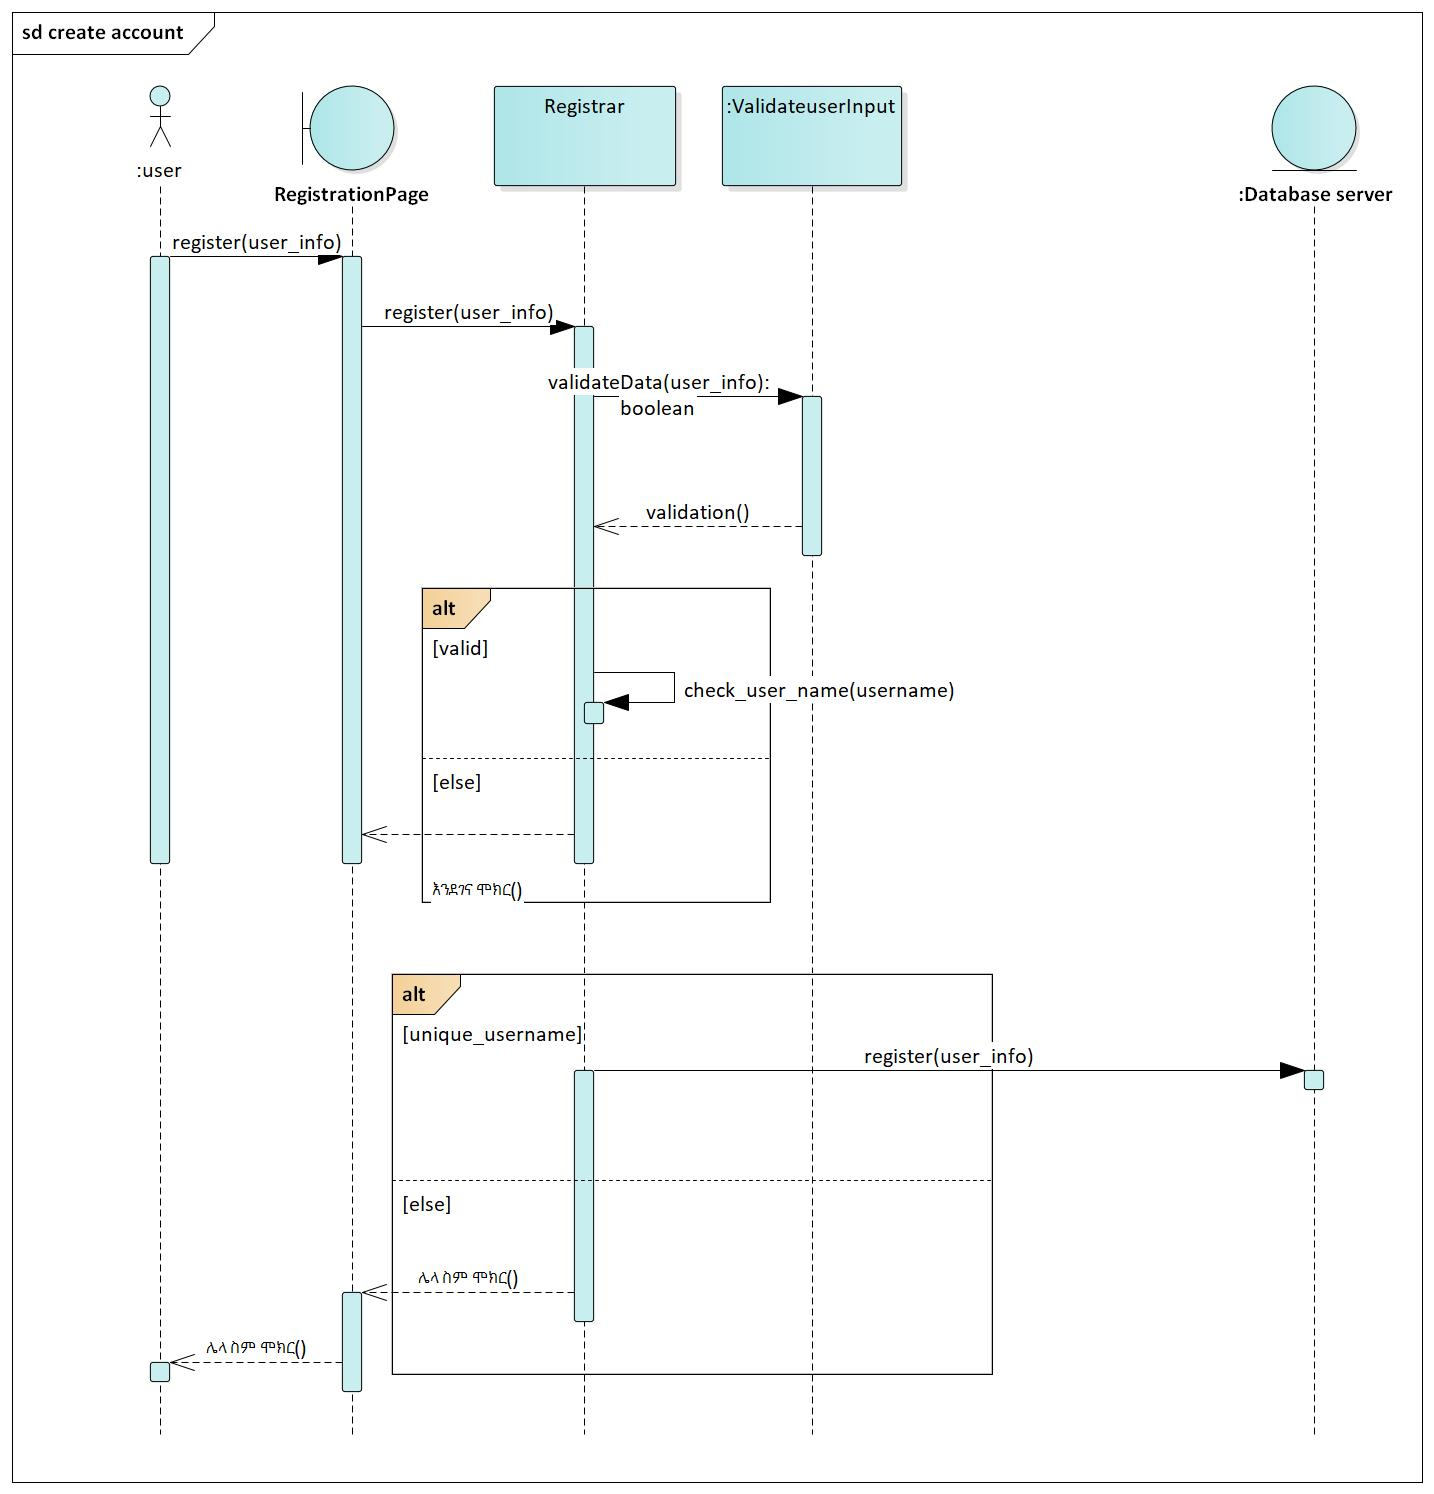
\includegraphics[width=15cm]{Diagram/sequence/Create Account.png}}
	\caption{Sequence diagram for creating account.}
	\label{dia_sqns_crtaccnt}

\end{center}
\end{figure}

\begin{figure}[H]
\begin{center}	

	\tcbox{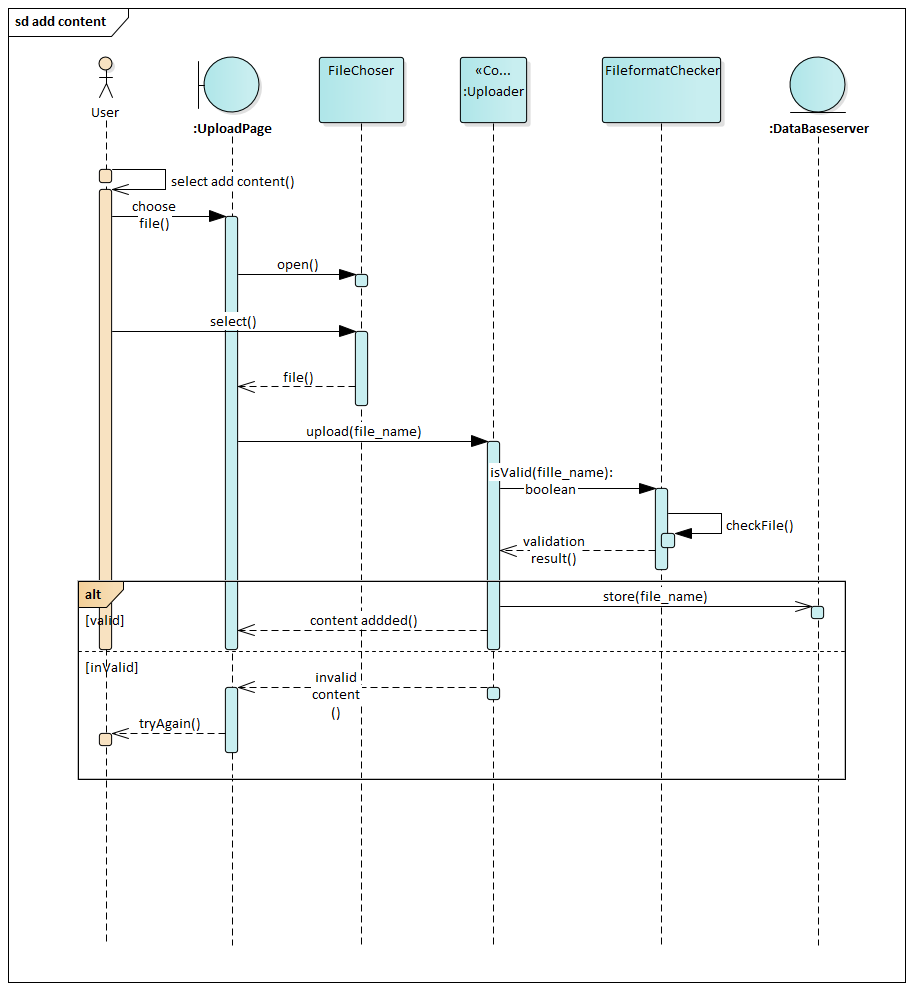
\includegraphics[width=15cm]{Diagram/sequence/Add Content.png}}
	\caption{Sequence diagram for adding content.}
	\label{dia_sqns_addcntnt}

\end{center}
\end{figure}


\begin{figure}[H]
\begin{center}	

	\tcbox{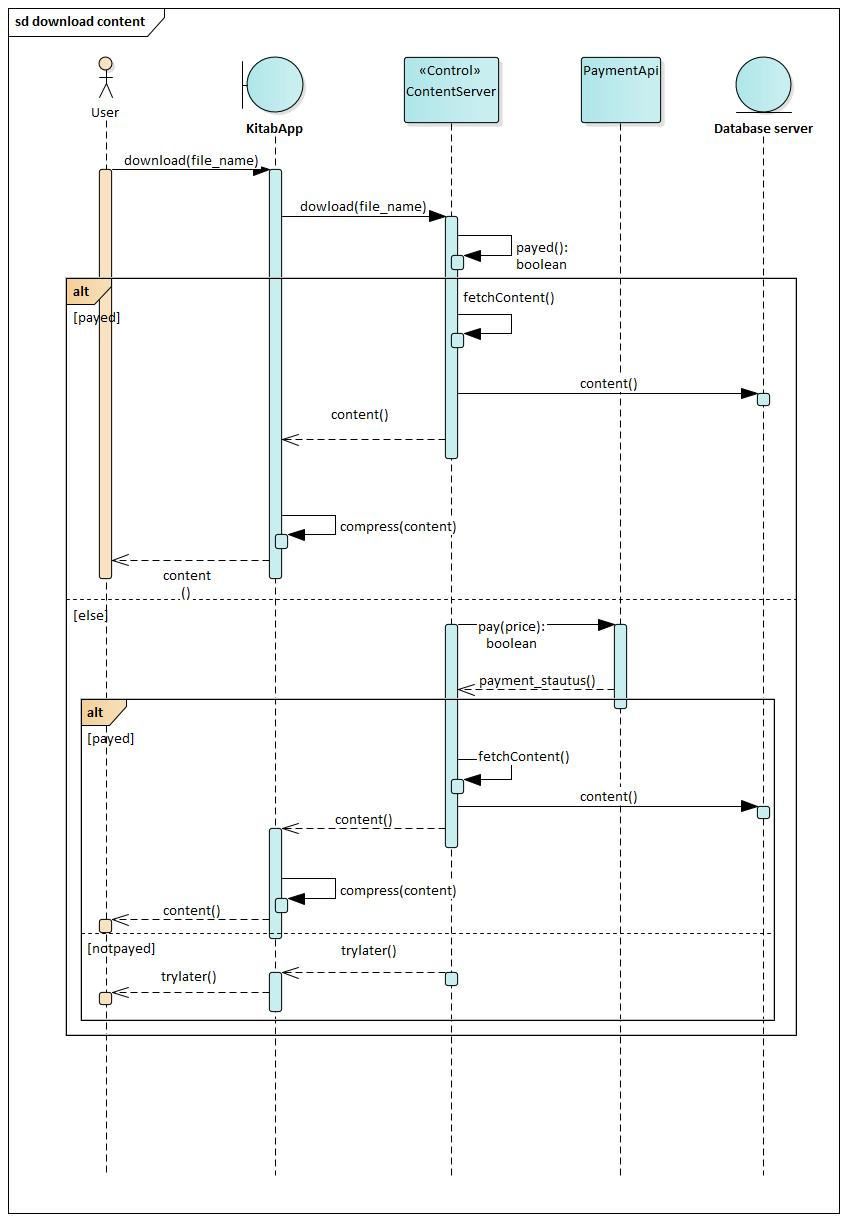
\includegraphics[width=15cm]{Diagram/sequence/Download Content.png}}
	\caption{Sequence diagram for downloading content.}
	\label{dia_sqns_dwnldcntnt}

\end{center}
\end{figure}

\begin{figure}[H]
\begin{center}	

	\tcbox{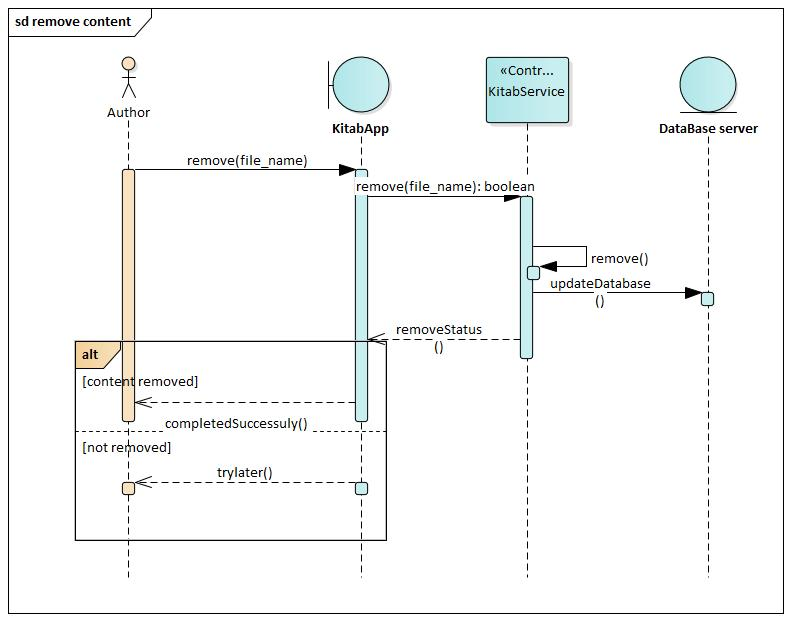
\includegraphics[width=15cm]{Diagram/sequence/Remove Content.png}}
	\caption{Sequence diagram for removing content.}
	\label{dia_sqns_rmvcntnt}

\end{center}
\end{figure}
